\chapter{ミラー計測実験}
\thispagestyle{empty}
\label{chap5}
\graphicspath{{chap5/figure/}}
\minitoc

\newpage
%%%%%%%%%%%%%%%%%%%%%%%%%%%%%%%%%%%%%%%%%%%%%%%%%%%%%%%%%%%%%%%%%%%%%%%%%%%%%


% ================================================== %
% section
% ================================================== %
\section{諸言}
\label{chap5_introduction}

本章では、実際に天文用Wolterミラーを\ref{chap3}章の提案手法による計測実験を行い、その解析を行う。
測定対象となるミラーは、2019年2月および同年9月に作製されたWolterミラーであり、それぞれについて位相回復計算を行った結果およびそこから計算される形状誤差について述べる。
また、これらは既に〇〇によって真円度測定がなされており、計測結果と真円度測定結果との比較・検討を行う。

\clearpage
% ================================================== %
% section
% ================================================== %
\newpage

\section{実験の構成}

実験装置の概要を図\ref{fig:mirror_experiment_schematic}に示す。
まず、レーザーからビームを出力し、これをNDフィルタによって減衰させ、強度を調整する。
次に、レンズを2つ使ってビームを拡大し平行化する。
これを測定対象のWolterミラーに入射し、さらにタイコグラフィのための回転ピンホールを通過させる。
最後に、一番下流にあるCCDカメラで強度分布を撮影する。

\begin{figure}[!ht]
\centering
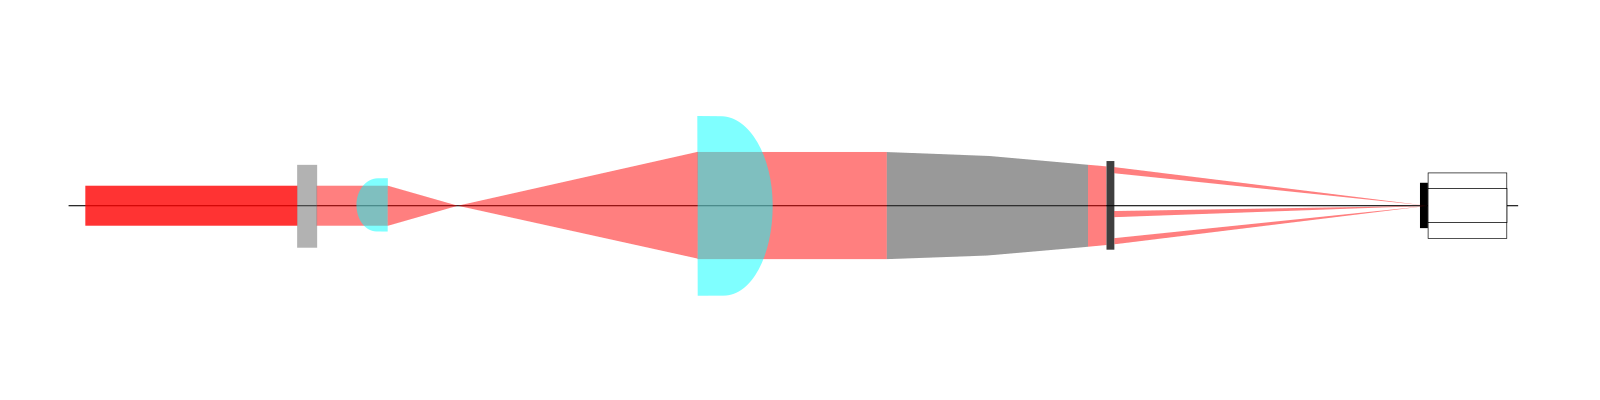
\includegraphics[width=14cm]{schematic.png}
\caption{ミラー測定実験系 模式図}
\label{fig:mirror_experiment_schematic}
\end{figure}

これらの光学素子のパラメータを表\ref{}に示す。
なお、NDフィルタは実験によってピークがダイナミックレンジに収まるよう適切に設定がなされるため、そのパラメータ等を記述しない。

\begin{table}[h]
\begin{center}
  \begin{tabular}{|c|c|} \hline
    パラメータ & 値 \\ \hline
    拡大用レンズ & 30.0 mm  \\
    拡大倍率 & 100 倍 \\
    設計波長 & 541.6 nm \\ \hline
  \end{tabular}
  \caption{Wolterミラー計測実験装置における各素子のパラメータ}
  \label{tb:mirror_experiment_params}
\end{center}
\end{table}

これらを構成した実験装置のCAD図を以下に示す。図\ref{fig:mirror_experiment_asm_cad_side}が横から見た図、図\ref{fig:mirror_experiment_asm_cad_isometric}が俯瞰して見た図である。

\begin{figure}[!ht]
\centering
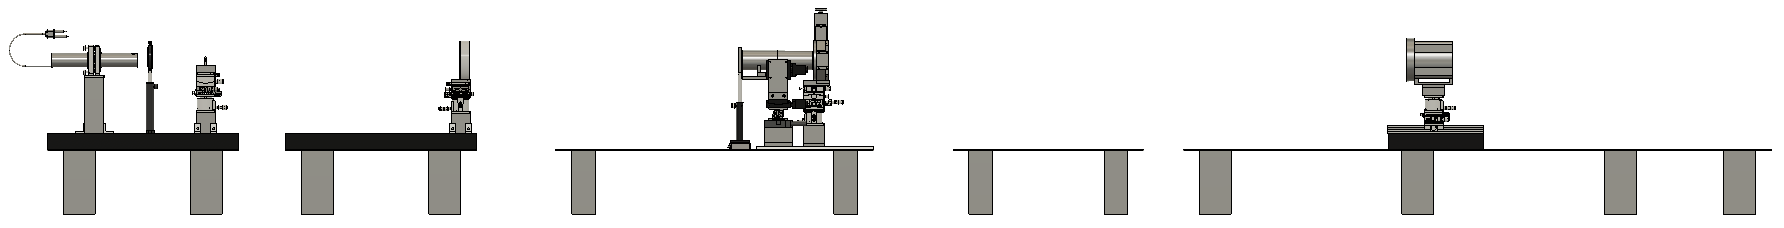
\includegraphics[width=14cm]{setup/asm_total_side.png}
\caption{ミラー測定実験系 側面図}
\label{fig:mirror_experiment_asm_cad_side}
\end{figure}

\begin{figure}[!ht]
\centering
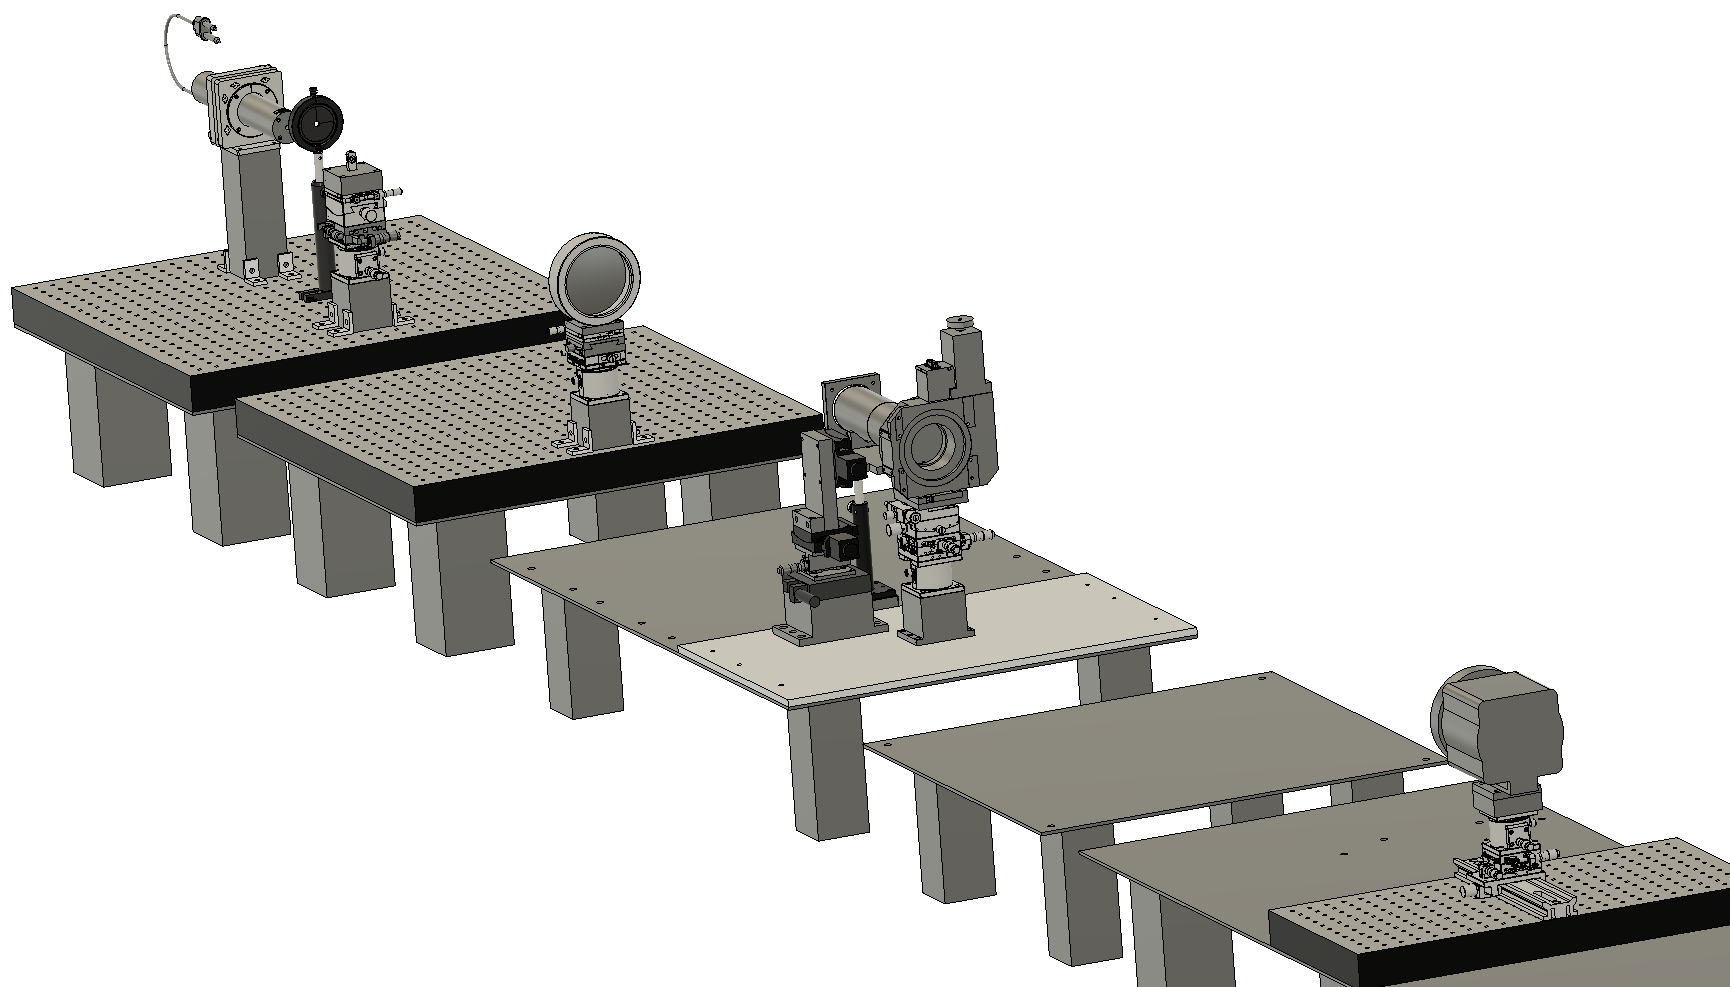
\includegraphics[width=10cm]{setup/asm_total_isometric.png}
\caption{ミラー測定実験系 俯瞰図}
\label{fig:mirror_experiment_asm_cad_isometric}
\end{figure}

\clearpage

% ================================================== %
% section
% ================================================== %
\newpage

\section{計測波面以外の通過光の処理方法に関する検討}
測定対象となっている天文用Wolterミラーは、X線集光用に設計・作製されたものであり、可視光を入射した際にどのような集光波面が生じるかは未検討である。
特に、可視光はX線に比べ2桁程度波長が長く、回折の影響が顕著であることが大きな差異として存在する。
\ref{chap4}章での提案手法の検討は、あくまで波面計測の対象である輪帯のみが存在する場合について行われたが、実際にミラーを計測する実験においては測定対象以外の光も通過してCCDカメラの方向に進行する。
円盤状に広がる平行光を入射した際にミラーより下流に通過する光は、図\ref{}に示す通り4種類存在する。
図\ref{}①が、測定対象となる波面、つまり正しく放物面、双曲面の順に2回反射した光である。
これに対して、図\ref{}②の直接通過してCCDカメラに到達する光、図\ref{}③の放物面に当たらず直接双曲面で反射された光、図\ref{}④の開口端のエッジで回折して進行する光が存在する。

\subsection{直接通過光}
直接通過光は、

\subsection{双曲面で1回反射した光}




\subsection{}
\label{chap5_}

\clearpage

% ================================================== %
% section
% ================================================== %
\newpage

\section{可視光ビームによるWolterミラー集光波面強度分布の測定}



\clearpage

% ================================================== %
% section
% ================================================== %
\newpage

\section{下流端走査タイコグラフィの結果}

\clearpage
% ================================================== %
% section
% ================================================== %
\newpage

\section{回復波面の解析}
\subsection{周方向誤差の真円度測定結果との比較}

% ================================================== %
% section
% ================================================== %
\section{結論}
\label{chap5_conclusion}


%%%%%%%%%%%%%%%%%%%%%%%%%%%%%%%%%%%%%%%%%%%%%%%%%%%%%%%%%%%%%%%%%%%%%%%%%%%%%

%%% Local Variables:
%%% mode: katex
%%% TeX-master: "../thesis"
%%% End:
